\documentclass[a4paper,twoside,titlepage,openright]{book}
\usepackage[MeX]{polski}
\usepackage[utf8]{inputenc}
\usepackage{enumitem} % słownik pojęć
\usepackage{amsmath}
\usepackage{tabularx} % tabele
\usepackage[usenames,dvipsnames,svgnames,table]{xcolor} % kolory jak się chce gdzieś użyć
\usepackage{graphicx} % żeby ryciny i zdjęcia były
\usepackage{listings} % syntax highlighting
\usepackage{verbatimbox} % marginesy dla tabel
\usepackage{emptypage} % usuwa nagłówki i numery stron z pustych stron

% PAGE LAYOUT
%\usepackage{showframe} % debug
\marginparwidth 0pt
\marginparsep 0pt
\usepackage[inner=4cm,outer=2cm]{geometry}

% HEADER, FOOTER
\usepackage{fancyhdr} 
\pagestyle{fancy}

% TABLE OF CONTENTS

%kropki w~spisie tresci
\makeatletter
\def\numberline#1{\hb@xt@\@tempdima{#1.\hfil}}
\makeatother

% CHAPTER TITLE

%kropki po tytułach rodziałów
\makeatletter
\def\@makechapterhead#1{%
  \vspace*{50\p@}%
  {\parindent \z@ \raggedright \normalfont
	\ifnum \c@secnumdepth >\m@ne
	  \if@mainmatter
	   \huge\bfseries \@chapapp\space \thechapter.
	   \par\nobreak
	   \vskip 20\p@
	\fi
   \fi
   \interlinepenalty\@M
   \Huge \bfseries #1\par\nobreak
   \vskip 40\p@
  }}
\makeatother

% SPIS TREŚCI

%kropki w~spisie tresci
\makeatletter
\def\numberline#1{\hb@xt@\@tempdima{#1.\hfil}}
\makeatother

% TYTUŁY ROZDZIAŁÓW

%kropki po tytułach rozdziałów
\makeatletter
\renewcommand*\@seccntformat[1]%
{\csname the#1\endcsname.\enspace}
\makeatother


% KONFIGURACJA WYGLĄDU NAGŁÓWKA TEGO CO SIĘ POWTARZA

\fancyhead{} 
\fancyhead[LE]{\rightmark}
\fancyhead[RO]{\leftmark}

% CODE LISTINGS 

\definecolor{mygreen}{rgb}{0,0.6,0}
\definecolor{mygray}{rgb}{0.5,0.5,0.5}
\definecolor{mymauve}{rgb}{0.58,0,0.82}

\lstset{ %
%frame=lines,
aboveskip=1.5em,
    belowcaptionskip=1.5em,
    xleftmargin=0.5cm,
  backgroundcolor=\color{white},   % choose the background color
  %basicstyle=\footnotesize,        % size of fonts used for the code
  breaklines=true,                 % automatic line breaking only at whitespace
  captionpos=b,                    % sets the caption-position to bottom
  commentstyle=\color{mygreen},    % comment style
  escapeinside={\%*}{*)},          % if you want to add LaTeX within your code
  keywordstyle=\color{blue},       % keyword style
  stringstyle=\color{mymauve},     % string literal style
}

\definecolor{maroon}{rgb}{0.5,0,0}
\definecolor{darkgreen}{rgb}{0,0.5,0}

\lstdefinelanguage{XML}
{
  basicstyle=\ttfamily,
  morestring=[s]{"}{"},
  morecomment=[s]{?}{?},
  morecomment=[s]{!--}{--},
  commentstyle=\color{darkgreen},
  moredelim=[s][\color{black}]{>}{<},
  moredelim=[s][\color{red}]{\ }{=},
  stringstyle=\color{blue},
  identifierstyle=\color{maroon},
  morekeywords={Page.DataContext,viewModel:NameViewModel}
}

%\setmonofont{Consolas} %to be used with XeLaTeX or LuaLaTeX
\definecolor{bluekeywords}{rgb}{0,0,1}
\definecolor{greencomments}{rgb}{0,0.5,0}
\definecolor{redstrings}{rgb}{0.64,0.08,0.08}
\definecolor{xmlcomments}{rgb}{0.5,0.5,0.5}
\definecolor{types}{rgb}{0.17,0.57,0.68}

\lstset{language=[Sharp]C,
%captionpos=b,
%numbers=left, %Nummerierung
%numberstyle=\tiny, % kleine Zeilennummern
%frame=lines, % Oberhalb und unterhalb des Listings ist eine Linie
showspaces=false,
showtabs=false,
breaklines=true,
showstringspaces=false,
breakatwhitespace=true,
escapeinside={(*@}{@*)},
commentstyle=\color{greencomments},
morekeywords={partial, var, value, get, set},
keywordstyle=\color{bluekeywords},
stringstyle=\color{redstrings},
basicstyle=\ttfamily\small,
}




\begin{document}

% ################################
%        STRONA TYTUŁOWA
% ################################

\begin{titlepage}

%\newgeometry{inner=3cm,outer=3cm}


\begin{center}
\begin{large}
Uniwersytet Mikołaja Kopernika\\[1mm]
Wydział Matematyki i~Informatyki\\[1mm]
\end{large}
\end{center}

\vfill

\begin{center}
{\Large Paweł Marcin Chojnacki}\\
nr albumu: 260082\\
informatyka
\end{center}

\vfill

\begin{center}
{\Large Praca inżynierska}
\end{center}

\vspace{0.5cm}

\begin{center}
{\Huge \textbf{Kopra -- aplikacja mobilna wspomagająca inwestowanie w~serwisie Kokos}}
\end{center}

\vspace{2cm}
\hfill
\begin{minipage}{6.5cm}
Opiekun pracy dyplomowej\\
dr Jerzy Białkowski
\end{minipage}

\vfill

\begin{center}
Toruń 2016
\end{center}

\end{titlepage}

% odwracamy kartkę ze stroną tytułową to nic nie ma z drugiej strony -> pusta strona
\clearpage{\pagestyle{empty}\cleardoublepage}

\tableofcontents

\chapter*{Słownik pojęć}
\markboth{}{Słownik pojęć}
\addcontentsline{toc}{chapter}{Słownik pojęć}
\begin{description}[style=nextline]
	\item[Aktywa finansowe] Środki finansowe przechowywane przez podmiot gospodarczy (osobę lub firmę), mające na celu przyniesienie w przyszłości korzyści ekonomicznych. Są to przechowywane środki pieniężne, umowy kredytowe, akcje innych firm.
	\item[Aukcja pożyczkowa] Oferta umowy pożyczkowej wystawiona przez pożyczkobiorcę, zweryfikowana na określonej platformie zgodnie z jej kryteriami. Oferta taka skierowana jest do wielu podmiotów określonych jako \textit{pożyczkodawców}.
	\item[Automat inwestycyjny] Oprogramowanie przeznaczone do symulowania działań pożyczkodawcy przez wpłacanie środków na aukcje spełniające określone kryteria.
	\item[FriendlyScore] Przyznanie punktacji użytkownikowi w oparciu o analizę danych z kont w serwisach społecznościowych, np. Facebooka czy Twittera oraz dodatkowe weryfikacje, np. weryfikację pracodawcy.
	\item[Giełda Papierów Wartościowych] Jest to instytucja publiczna zapewniająca możliwość obrotu giełdowymi papierami wartościowymi. Pozwala ona na kupno oraz sprzedaż papierów wartościowych takich jak akcje i obligacje. W mojej pracy ograniczę się do polskiego rynku kapitałowego, dlatego pojęcie ,,Giełda Papierów Wartościowych'' (w skrócie ,,Giełda'') będzie w niej oznaczać instytucję „Giełda Papierów Wartościowych w Warszawie SA”.
%	\item[Inteligencja finansowa] Pojęcie nie zostało zdefiniowane przez Słownik Języka Polskiego, jednak szeroko używane w ,,poradnikach'' finansowych, blogach czy książkach nt. rozwoju osobistego. Oznacza sprawne posługiwanie się finansami, zrozumienie podstawowych zasad matematyki, tj. procent, procent składany, porównywanie liczb czy obliczanie wartości prostych szerów, ciągów. Zbiór umiejętności tak oczywisty dla matematyków, że nie wpadli by nazwać go ,,inteligencją''.
	\item[Instrument finansowy \textit{(ang. financial instrument)}]  Jest to kontrakt zawarty między dwiema stronami regulujący zależność finansową między tymi stronami. W tym kontrakcie zawarte są dwie strony. Strona długa \textit{(ang. long party)}, inaczej -- posiadacz długiej pozycji, oraz strona krótka \textit{(short party)}, inaczej -- posiadacz krótkiej pozycji. Przykładem instrumentu finansowego są papiery wartościowe. \cite{inwestycje}
	\item[Instytucja finansowa] Podmiot gospodarczy, który zajmuje się obrotem środków finansowych powierzonych przez klientów (udzielanie kredytów, inwestycje, gromadzenie środków pieniężnych).
	\item[Oferta inwestycyjna] Przekazanie wkładu pieniężnego na wybraną pożyczkę przez jednego z pożyczkodawców. Wiąże się to ze wstępną akceptacją oferty pożyczkowej na warunkach wcześniej określonych przez osobę wystawiającą aukcję pożyczkową \textit{(pożyczkobiorcę)}.
	\item[Pożyczka] Przekazanie określonemu podmiotowi podmiotu pieniędzy na określony czas z zastrzeżonym terminem zwrotu. 
	\item[Pożyczka społecznościowa \textit{(ang. social lending)}] Pożyczka wykonywana bezpośrednio pomiędzy osobami fizycznymi poprzez serwisy internetowe, bez pośrednictwa instytucji finansowych.
	\item[Pożyczkobiorca] Osoba lub instytucja biorąca pożyczkę.\cite{slownikPwn}
	\item[Pożyczkodawca] Osoba lub instytucja udzielająca pożyczki.\cite{slownikPwn}
	\item[RRSO (Rzeczywista roczna stopa oprocentowania)] Wszystkie koszty realnie ponoszone przez pożyczkobiorcę. Kwotę wyraża się w wartości procentowej całkowitej kwoty kredytu w stosunku rocznym. (Przykładowo, Tomek, pożyczając 1000~zł na 2~lata musi oddać 1200 zł. Roczna opłata za kredyt wynosi $ 200 / 2 = 100 \text{ zł} $, co jest wartością 10\% z całkowitej pożyczonej kwoty. RRSO wynosi wtedy 10\%.)
	\item[Saldo] Stan konta w wybranej walucie lub jednostce aktywów (ilość akcji, kruszcu), po uwzględnieniu wszystkich transakcji rozliczonych i nierozliczonych w danej chwili.
	\item[Toksyczne aktywa] Aktywa finansowe, których ryzyko inwestycyjne zostało pierwotnie istotnie niedoszacowane przez posiadacza. Przeważnie są to papiery wartościowe oraz pożyczki obarczone wysokim ryzykiem kredytowym lub płynności, którego realizacja może skutkować poważnym pogorszeniem sytuacji finansowej posiadacza i w efekcie jego upadłością.\cite{slownikNBP}
	\item[Windykacja] Dochodzenie własności za pomocą dostępnych środków prawnych. Dążenie do odzyskania pieniędzy przekazanych podmiotowi przez osobę wszczynającą proces odzyskiwania należności.
	\item[Zobowiązania] Zmuszenie prawem do świadczenia pieniężnego na rzecz wierzyciela.
\end{description}
 
\chapter*{Wstęp}
\markboth{}{Wstęp}
\addcontentsline{toc}{chapter}{Wstęp}

\section*{Pomysł napisania aplikacji o tematyce finansowej}
\addcontentsline{toc}{section}{Pomysł napisania aplikacji o tematyce finansowej}

Od 2010 roku interesuję się tematyką oszczędzania pieniędzy i pomnażania oszczędności. Początkowo starałem się szukać bezpiecznego miejsca dla oszczędności w lokatach, które do 2012 roku jeszcze przebijały inflację. Lokaty jednodniowe, potocznie znane jako ,,antybelki'', były popularnym sposobem na ominięcie podatku od dochodów kapitałowych. Po kilkukrotnej inwestycji w lokaty, zauważyłem, że większy zysk można osiągnąć odkładając kapitał na Giełdzie Papierów Wartościowych. Szybka lektura na temat podstaw inwestowania w papiery wartościowe okazała się być dla mnie lekcją pokory. Jeśli zacznę inwestować bez poświęcenia wielu godzin na naukę funkcjonowania giełdy, stracę wszystkie oszczędności. Inwestowanie w akcje jest obarczone wysokim ryzykiem. Wymaga praktyki, wiedzy i ciągłego obserwacji sytuacji na rynku. Nie byłem skory do zmiany planów życia, by wyciągnąć trochę więcej z moich oszczędności. 

Szukając w internecie innych możliwości inwestycji natknąłem się na względnie nowy produkt na polskim rynku. Są nim pożyczki społecznościowe -- prosta idea wykorzystująca zestaw technologii znany jako Web 2.0. Zawartość serwisu tworzą użytkownicy. Pożyczając sobie wzajemnie pieniądze, omijają banki i zarabiają pieniądze na klasycznych umowach pożyczkowych. Zalety tego rozwiązania, takie jak zysk z inwestycji wyższy niż na lokatach bankowych oraz bardzo niska krzywa nauki, zachęciły mnie do wkroczenia w świat kredytów. Już ponad 6 lat odkładam nadmiar gotówki z przyzwoitym wynikiem, który po uśrednieniu przekracza maksymalny możliwy zysk z lokaty bankowej. 

Gdybym posiadał ciągły dostęp do serwisu, osiągnąłbym dużo wyższy zwrot z inwestycji, ponieważ wiedziałbym, kiedy pojawia się tzw. gorąca oferta (pożyczka na bardzo dobrych warunkach, zazwyczaj jest zamykana w ciągu godziny od założenia aukcji). Jednak nie byłbym w stanie poświęcić całego dnia na przeglądanie wszystkich ofert. \textbf{Mogę natomiast napisać aplikację mobilną, która poinformuje mnie, gdy nadarzy się okazja godna odciągnięcia od innych obowiązków.} 

Zdaję sobie sprawę, że również inni inwestorzy często wspominają, jak sprzed nosa uciekały im prawdziwe żyły złota -- tylko dlatego że nie mieli ciągłego dostępu do strumienia informacji. Biorąc pod uwagę zainteresowanie wokół problematyki, uważam, że temat mojej pracy inżynierskiej znajduje praktyczne zastosowanie i nie jest tylko sztuką dla sztuki. Uważam go za projekt z potencjałem do dalszego rozwoju. Wybrałem temat, który mnie interesuje, czyli instrumenty finansowe. Są one nie tylko bardzo ciekawym lecz także istotnym zagadnieniem. Jest to szczególnie widoczne, gdy spojrzy się na nie z szerszej perspektywy -- np. przez pryzmat skutków społeczno-ekonomicznych, jakie można spowodować przez manipulacje rynkami finansowymi. Jedna osoba, operując sporymi ilościami aktywów, jest w stanie znacząco zmienić gospodarkę całego kraju. Przykładem na to są działania George Sorosa, który na spekulacjach walutowych wyprowadził ponad 1~miliard funtów brytyjskich.\cite{soros}

Niniejsza praca skupia się wokół rynku pożyczek finansowych, gdzie występują niewielkie obroty gotówkowe w przeliczeniu na osobę. Ze względu na swój mikro charakter pożyczki społecznościowe cieszą się moim szczególnym uznaniem. Uważam, że pomagają jednostkom wyjść z problemów ekonomicznych, a w wielu przypadkach urzeczywistniają wizję samodzielnego podnoszenia stopy życia. Zalet pożyczek opartych na społecznościach jest wiele. Przedstawiam je w dalszych rozdziałach, zestawiając razem z wadami i ryzykiem inwestycyjnym.

\section*{Podobne rozwiązania w świecie aplikacji mobilnych}
\addcontentsline{toc}{section}{Podobne rozwiązania w świecie aplikacji mobilnych}

Przeanalizowałem rynek aplikacji mobilnych w sklepach: Google Play, App Store, Windows Store, Amazon AppStore oraz F-Droid. W sklepie Google Play znalazłem jedną aktywnie rozwijaną aplikację wspomagającą pożyczki społecznościowe -- Kokoid. Jest to nowa aplikacja (z początku 2016 roku), przeznaczona na system Android. Swój model biznesowy opiera na wyświetlaniu reklam w trakcie działania.

Oprogramowanie wspomagające inwestycje istnieje głównie w formie aplikacji internetowych. Popularnym narzędziem wspomagającym pożyczkodawców jest www.zndpd.pl czyli \textit{,,Zestaw Narzędzi Pożyczkodawców''}. Stanowi ono rozbudowane narzędzie umożliwiające przeglądanie informacji o aukcjach, pożyczkobiorcach i statystykach spłacalności z różnych serwisów. Wszystkie dane zebrane są jednym miejscu w formie strony z raportem. Funkcjonalność portalu zorientowana jest na wyświetlaniu statystyk i generowaniu raportów dotyczących własnych inwestycji.

Nie dostrzegłem żadnych aplikacji o podobnej tematyce (przynajmniej na polskim rynku), na których mógłbym się wzorować. Z tego powodu większość zaimplementowanych funkcjonalności to pomysły nowe, gotowe do przetestowania poza środowiskiem deweloperskim.

\section*{Rozważane formy wdrożenia projektu}
\addcontentsline{toc}{section}{Rozważane formy wdrożenia projektu}

Najlepsze rozwiązanie pod względem satysfakcji użytkownika końcowego stanowi stworzenie zestawu narzędzi w formie aplikacji internetowej. Aplikacja ta udostępniałaby API dla aplikacji mobilnych lub aplikacji przeglądarkowej. Główną zaletą tego pomysłu jest dostęp do usługi niezależnie od posiadanej platformy mobilnej. Dodatkowo istnieje możliwość dostosowania danej aplikacji mobilnej do ergonomii wskazanego systemu operacyjnego, co zapewniłoby najwyższą wygodę użytkowania. 

Niestety wdrożenie tej idei byłoby zbyt pracochłonne na jednoosobowy projekt. Aby go wdrożyć, należałoby zastosować podział na kilka niezależnych komponentów, wśród których każdy wykorzystywałby inne technologie. Zazwyczaj takie projekty realizowane są we współpracy wielu specjalistów z różnych dziedzin.

Z powyższych względów, najlepszym sposobem na zrealizowanie pomysłu jest napisanie prostej aplikacji mobilnej działającej pod kontrolą systemu Windows Phone 8.1. 

Czynniki, które zdecydowały o implementacji projektu w formie aplikacji to: zajęcia z programowania Windows Phone, znajomość platformy .NET, doświadczenie w tworzeniu interfejsów użytkownika z wykorzystaniem XAML'a.

\section*{Jaki jest cel aplikacji?}
\addcontentsline{toc}{section}{Jaki jest cel aplikacji?}

Zależy mi, by osoba korzystająca z aplikacji mogła w każdej chwili przeglądać najważniejsze informacje o wybranych przez siebie aukcjach, a także dowiadywać się w czasie rzeczywistym o nowych ofertach pożyczkowych. Umożliwi jej to w ciągu kilku godzin podjąć decyzję o nowej inwestycji. Celem zasadniczym jest \textbf{skrócenie czasu potrzebnego do podpisania umowy o pożyczkę}. By tego dokonać, zaprezentuję inwestorowi najistotniejsze dane. Przypomnę, gdy zajdzie potrzeba, że pojawiła się kolejna oferta oraz pozwolę wyszukać aukcje, które najbardziej interesują inwestora.

\section*{Założenia projektowe}
\addcontentsline{toc}{section}{Założenia projektowe}

Cała praca skupia się na ułatwieniu dostępu do korzystania z najpopularniejszego serwisu pożyczek społecznościowych w Polsce. Aplikacja ma być bezpieczna, stabilna, niezawodna. Szybkość działania jest kwestią drugorzędną, gdyż aplikacja operuje na zbyt małych zbiorach danych, by ich przetwarzanie miało powodować znaczące spowolnienia w responsywności. Myślą przewodnią jest dostarczenie wyłuskanych informacji w odpowiednim momencie. 

Kopra jest zgodna z wytycznymi Microsoftu dot. projektowania aplikacji mobilnych dla systemu Windows Phone: \textit{,,Aplikacja ma robić jedną rzecz i ma ją robić dobrze''}\cite{wpDesign} oraz \textit{,,Do more''}\cite{doMore}. Oba hasła odnoszą się do skupienia na produktywności i komforcie użytkownika. 

\section*{Korzystanie z serwisów pożyczkowych na smartfonach}
\addcontentsline{toc}{section}{Korzystanie z serwisów pożyczkowych na smartfonach}

Na polskim rynku nie istnieje obecnie żadne rozwiązanie łączące świat mobilny z rynkiem pożyczek społecznościowych. Brak natychmiastowego dostępu do własnych inwestycji wywołuje stres i zniechęca do poważnej aktywności, ponieważ decyzje powinny być podejmowane jak najkrótszym czasie. 

Poszukiwanie nowych ofert na przeglądarce telefonu jest bardzo niewygodne. Ponadto korzystanie na małym ekranie ze starych, nieresponsywnych interfejsów serwisów internetowych wymaga od użytkownika wiele cierpliwości. Instytucje finansowe nie wprowadzają ułatwień dostępu dla urządzeń mobilnych. 

Jako osoba inwestująca wziąłem sprawy we własne ręce i stworzyłem aplikację mobilną. Teraz, aby uzyskać dostęp do najnowszych okazji pożyczkowych, wystarczy posiadać urządzenie wyposażone w system operacyjny Windows Phone 8.1 lub nowszy oraz połączenie z internetem.

Uważam, że Kopra ułatwi użytkownikom systemu Windows Phone 8.1 szybki dostęp do informacji.




\clearpage{\pagestyle{empty}\cleardoublepage}
\chapter{O pożyczaniu}
\section{Krótka historia pieniądza}
Pożyczki istnieją od tysięcy lat. Pierwsze informacje o pożyczaniu pieniędzy wywodzą się ze starożytnej Mezopotamii \cite{financingCivilization}. 

Zajęcie było to tak popularne, że grupy osób zaczęły się specjalizować w pośrednictwie między tymi, którzy mieli pieniądze oraz tymi, którzy te pieniądze chcieli pożyczyć. Dzisiaj te grupy stanowią banki. 

Wypaczając ideę pożyczania pieniędzy od osób posiadających pieniądze (pożyczkodawców) do osób biorących te pieniądze na pewien czas (pożyczkobiorców), banki stały się przedsiębiorstwami szukającymi zysków na obrocie pieniędzmi -- nie tylko na ich pożyczaniu. Doprowadziło to do bardzo wielu niebezpiecznych zachowań. 

Najgorszym z nich jest \textbf{system rezerw cząstkowych}. Działa on poprawnie do czasu, kiedy następuje zalanie rynku \textbf{toksycznymi pożyczkami}. Jednakże gdy to nastąpi, bank nie jest w stanie utrzymać płynności finansowej. Okazuje się wówczas, że większość jego pieniędzy to zabezpieczenia bez pokrycia, których nie da się wyegzekwować. 

Kolejnym niebezpieczeństwem, jakie niesie ze sobą system rezerw cząstkowych, jest stałe zagrożenie wahaniami nastrojów społecznych. W wyniku plotki rozpuszczonej wśród klientów banku bądź też czasowej niewypłacalności depozytów może nastąpić \textbf{zjawisko paniki bankowej}. Wielu ekonomistów zgadza się z poglądem, iż dobrze zarządzany system rezerw cząstkowych prowadzi do szybszego rozwoju gospodarczego i uniezależnia bogactwo kraju od złóż naturalnych.\cite{fractionalReserveBanking}

\section{Idea pożyczek społecznościowych}
Pożyczki społecznościowe w języku angielskim znane są jako \textit{,,peer-to-peer lending''} (w skrócie: P2P). Jest to zbiór czynności polegających na korelowaniu osób potrzebujących kredytu gotówkowego z ludźmi chętnymi do udzielenia części kredytu przez platformę online.\cite{P2P} 

Dla osób z dodatkową gotówką jest to sposób na naukę oceny ryzyka inwestycji niewielkim kosztem (stawki wejściowe do inwestycji są bardzo niskie). Szczególną zachętą jest tutaj relatywnie duży zwrot z inwestycji biorąc pod uwagę współczynnik ryzyka. 

W Polsce serwisy pożyczek społecznościowych upowszechniły się, kiedy oprocentowanie lokat spadło poniżej 5\% (zaraz po zablokowaniu lokat jednodniowych).\cite{antybelkowe} Spowodowało to nagły wzrost zainteresowania rynkiem pożyczek -- wliczając w to mniej bezpieczne umowy z wyższym oprocentowaniem. Doprowadziło to do sytuacji obniżenia oprocentowania pożyczek kwalifikowanych jako ,,wysokiego ryzyka'', czyli takich o wyższej niespłacalności przy stosunkowo niskim oprocentowaniu. Sytuacja po roku ustabilizowała się. 

Ostatecznie wszystkie serwisy pożyczek społecznościowych w Polsce poprawiły wymogi weryfikacji finansowej w celu udzielenia pożyczki. Ponadto oprocentowanie maksymalne zostało obniżone z 25\% do 10\% (stan na październik 2016). W efekcie instrumenty te stały się niewiele bardziej opłacalne od lokat sprzed czasów ustawy blokującej omijanie podatku od dochodów kapitałowych.
 
 
\section{Ryzyka związane z pożyczkami społecznościowymi}

Jako ryzyka związane z inwestowaniem w rynek pożyczek można wymienić:

\begin{itemize}
\item sprzeczne interpretacje prawne Naczelnego Sądu Administracyjnego przy czerpaniu zysków z pożyczek społecznościowych,
\item problemy ze ściąganiem wierzytelności.
\end{itemize}

W akapitach poniżej znajduje się krótkie omówienie tych problemów oraz sposoby rozwiązania ich.

\subsection*{Urząd Skarbowy}
Zyski z przychodów kapitałowych są opodatkowane 19-procentową stawką (na rok 2016). Jedyną jasną kwestią jest to, iż od każdego wypracowanego zysku należy zapłacić podatek. 

Problem pojawia się z interpretacją prawa -- kiedy należy założyć działalność gospodarczą oraz w jaki sposób rozliczać się z Urzędem Skarbowym i fiskusem. Naczelny Sąd Administracyjny w sprawie o sygnaturze II FSK 1472/10 orzekł, że regularne inwestowanie w pożyczki nosi znamiona działalności gospodarczej.\cite{nsaZnamiona} Jednak w sprawie o sygnaturze II FSK 142/10 ten sam sąd wydał wyrok odwrotny, uznając wówczas, że pożyczanie pieniędzy nie nosi znamion prowadzenia działalności gospodarczej. \cite{nsaWyrokOdwrotny} 

Mając na uwadze powyższe wyroki, przed rozpoczęciem regularnego pożyczania, \emph{należy zwrócić się do dyrektora właściwej sobie Izby Skarbowej z zapytaniem o sposób rozliczania.} \cite{oswiadczenieKokos}

\subsection*{Windykacja}

Jak wygląda odzyskiwanie wierzytelności przy braku spłat? Pierwszą rzeczą, którą należy zrobić to próbować rozmowy z wierzycielem, wyjaśnić przyczyny opóźnień i znaleźć sposób na najszybszy powrót do regularnych spłat. 

Jeśli kontaktu nie można nawiązać natychmiast, można skorzystać udostępnionych w serwisach monitów. Monit jest przypomnieniem o zaległych ratach, wysyłanym w formie SMS/telefonu/wiadomości email. Jednakże dla spłacającego monit stanowi dodatkowe obciążenie finansowe, dlatego nie jest to rozwiązanie zalecane jako pierwsza forma ,,kontaktu''. 

Kolejny krok stanowi podjęcie działań prawnych. Na tym etapie zaczynają się problemy dla inwestora, gdyż musi podjąć decyzję, czy ściągać należności samodzielnie, wynająć firmę prawniczą lub też skorzystać z usług windykacyjnych dostępnych w serwisie. 

Dobrym rozwiązaniem jest wspólna windykacja większości pożyczkodawców aukcji. Polega ona na tym, że inwestorzy wspólnie wynajmują firmę windykacyjną, gdzie za 10-15\% odzyskanej kwoty mogą liczyć na większe prawdopodobieństwo odzyskania pieniędzy. Jeśli firma nie odzyska długu, nie dostaje wynagrodzenia.


\section{Jakie zyski można osiągnąć?}

\textbf{Średnie oprocentowanie} w serwisie Kokos wynosi 16,87\% \cite{zostanInwestorem} (na dzień 28.10.2016).

\textbf{Stopa lombardowa} ustalona przez Narodowy Bank Polski wynosi 2,5\% \cite{stopy} (ustalona w dniu 05.03.2015).
 
\textbf{Maksymalne oprocentowanie} dla pożyczki w skali roku to stawka stopy lombardowej pomnożona razy cztery, czyli 10\%.

Średnie oprocentowanie w serwisie jest wyższe niż 10\%, ponieważ jest liczone od czasu powstania serwisu, kiedy to stawka lombardowa wynosiła 6,25\%, co dawało maksymalny zysk do 25\% rocznie. Stawka oprocentowania rośnie również wówczas kiedy pożyczka zostaje spłacona przed czasem. Jest to możliwe szczególnie w przypadku gdy PB buduje swoją reputację i zobowiązuje się spłacić 3-letnie zobowiązanie w ciągu 1 roku. 

Z moich osobistych obserwacji wyłania się obraz zwrotu z inwestycji na poziomie 12\% rocznie, wliczając w to niespłacone zobowiązania. Warto zauważyć, iż w trakcie całej operacji inwestujemy także swój czas. Rozważając opłacalność pożyczek społecznościowych należy wliczyć również czas poświęcony na analizę i pilnowanie inwestycji oraz czas na kontaktowanie się z pożyczkobiorcą i innymi wpłacającymi. Zysk przekraczający zainwestowany czas można zaobserwować przy kwotach inwestycji powyżej 500~zł miesięcznie. 

Utrzymywanie się z odsetek zarobionych na pożyczkach wymaga pełnoetatowego zaangażowania w zarządzanie narastającą ilością pożyczek. W takim przypadku można zająć się również inwestowaniem w akcje.


\section{Porównanie najpopularniejszych instrumentów finansowych}

% będziesz chciał sobie robić kolory, to można tak:
% \cellcolor[HTML]{D8FF91}

Zysk rośnie wraz z ryzykiem. Przy inwestowaniu aktywów zawsze istnieje ryzyko straty części lub całości inwestycji. Można zaobserwować niemal wykładniczą zależność między ryzykiem utraty inwestycji, a wysokością osiągniętych zysków. 

Poniżej prezentuję prostą tabelę z porównaniem przykładowych zysków i ryzyka dla poszczególnych instrumentów finansowych. 

\begin{small}
\noindent
\addvbuffer[12pt 0pt]{\begin{tabularx}{\textwidth}{@{}|l| *6{>{\centering\arraybackslash}X|}@{}}
  \hline
  \textit{Właściwość} & \textbf{Obligacje} & \textbf{Lokata} & \textbf{Fundusz inwestycyjny} & \textbf{Pożyczka społecznościowa} & \textbf{Giełda} \\
  \hline 
  \textbf{Ryzyko} & Brak & Brak & Niskie & Średnie & Wysokie \\
  \hline
  \textbf{Rentowność} & Znikoma & Niska & Średnia & Średnia, Wysoka & Wysoka \\
  \hline
  \textbf{Czas inwestycji} & Min. 60 mies. & 3--12 mies. & Min. 60 mies. & 12--36 mies. & Min. 36 mies. \\
  \hline
  \textbf{Poziom skomplikowania} & Podstawowy & Podstawowy & Łatwy & Średni & Wysoki \\
  \hline
\end{tabularx}}
\end{small}


\section{Porównanie polskich serwisów pożyczkowych}

Istniejące serwisy w Polsce to:

\begin{enumerate}

	\item Finansowo.pl \cite{finansowoPl}
	\item Zakra.pl \cite{zakraPl}
	\item Kokos.pl \cite{kokosPl}
	\item Lendico.pl \cite{lendicoPl}
	\item Zakramini.pl \cite{zakraminiPl}
	\item AppleCredit.pl \cite{applecreditPl}
	\item CapitalClub.pl \cite{capitalclubPl}

\end{enumerate}

\begin{small}
\noindent
\addvbuffer[8pt 12pt]{\begin{tabularx}{\textwidth}{@{}|l| *7{>{\centering\arraybackslash}X|}@{}}
   \hline
   \textit{Serwis} & \textbf{Użytko-wnicy} & \textbf{Udzielone pożyczki} & \textbf{Spłacone zobowiązania} & \textbf{Spłacalność} & \textbf{Średnie oprocentowanie} & \textbf{Charakter} \\
   \hline
   \textbf{Finansowo} & b/d & b/d & 85 813 tys. zł & 91,9\% & 5,49\% & Chwilówki \\
   \hline
   \textbf{Zakra} & 39 tys. & b/d & b/d & b/d & 10\% & Konsument\\
   \hline
   \textbf{Kokos} & 309 tys. & 126 tys. & 144 426 tys. zł & 93\% & 16,86\% & Konsument \\
   \hline
   \textbf{Zakramini} & 17 tys. & 44 tys. & 13 706 tys. zł & b/d & b/d & Chwilówki \\
   \hline
   \textbf{AppleCredit} & 8 tys. & 2 tys. & 1 135 tys. zł & b/d & 9\% & Chwilówki \\
   \hline
   \textbf{CapitalClub} & 1 tys. & 0,1 tys. & 4 000 tys. & b/d & b/d & Inwestycje \\
   \hline
\end{tabularx}}
\end{small}

W zestawieniu brakuje serwisu Lendico. Ten niemiecki serwis zawiesił działalność inwestycyjną -- od kilku miesięcy nie ma ofert inwestycyjnych. Jest prawdopodobne, że ze względu na niskie zainteresowanie zostanie wkrótce wycofany z polskiego rynku.

\section{Wybór systemu do implementacji}

Pierwszym i obecnie najpopularniejszym serwisem jest \textbf{Kokos}. W ciągu 8~lat działalności pożyczono 143,4mln zł na 126~738 aukcjach. Dla porównania, CapitalClub informuje na stronie głównej o sumie 4~mln~zł przez 102~udzielone pożyczki dla firm. 

Kokos, którego właścicielem jest firma Bluemedia, posiada:
\begin{itemize}
\item największą bazę aktywnych inwestorów,
\item wiele innowacyjnych zabezpieczeń, takich jak np. FriendlyScore,
\item responsywny interfejs,
\item przelewy ekspresowe,
\item raporty inwestora,
\item podstawowe API do zapytań o aukcję.
\end{itemize}

Ważnym aspektem jest również \textbf{dostęp do interfejsu programistycznego udostępnionego dla programistów}. Ze wszystkich platform, API jest udostępnione na trzech – Kokos, Zakra, Zakramini. 

Zakra i Zakramini pozwalają korzystać programiście lub inwestorowi z zapytań do serwisu po osobistej prośbie o wygenerowanie klucza. Stanowi to wielką przeszkodę, gdyż każdy kto chce sprawdzić działanie funkcjonalności jest zobowiązany wystosować pisemną prośbę o wygenerowanie klucza i otrzyma dostęp do WebAPI dopiero po upływie kilku dni. 

Kolejnym mankamentem jest bardzo okrojony zakres zwracanych informacji. Dostępne są następujące wywołania (wraz z odpowiedziami):

\begin{description}[style=nextline]

	\item[getUserData(id użytkownika)] [id użytkownika, nazwa użytkownika, rok urodzenia, miasto zameldowania, id użytkownika w serwisie Zakramini, nazwa użytkownika w serwisie Zakramini, kwota zadłużenia w serwisie Zakramini, czas opóźnień spłaty na w serwisie Zakramini]
	
	\item[getAuctionData(id aukcji)] [id, id pożyczkobiorcy, oprocentowanie, kwota pożyczki, numer aukcji, bonus pożyczkodawcy, status aukcji, data utworzenia]
	
	\item[getRunningLoansFromUser(id użytkownika)] [tablica z aukcjami jak getAuctionData]
	
	\item[getAuctionInstallmentsData(id aukcji)] [id aukcji, dzień płatności, data pierwszej spłaty, ilość spłaconych rat, ilość zaległych rat]

\end{description}

Zwracają one tylko najbardziej podstawowe informacje \cite{zakraPlApi}, właściwie szczątkowe. Nie można z nich złożyć porządnej informacji kredytowej.

Pozostaje jeszcze Kokos ze swoim interfejsem. Pozwala na uzyskanie znacznie bardziej złożonych informacji o aukcji, użytkownikach, stanie finansowym. Wygenerowanie klucza jest niesamowicie proste -- wystarczy kliknięcie w przycisk ,,Wygeneruj klucz'' i od razu otrzymujemy klucz aktywny przez rok. 

Mam nadzieję, że po przedstawieniu powyższych informacji jest jasne, że wybór, który serwis obsłużyć, tak naprawdę nie istnieje.

\section{WebAPI}

Interfejs programistyczny wchodzi w skład narzędzi użytkowników. Dokumentacja \cite{kokosPlApi} jest prawie kompletna (parę brakujących elementów można szybko wywnioskować z kontekstu). 

Aby rozpocząć korzystanie, należy wygenerować własny klucz i zapoznać się z regulaminem korzystania oraz dokumentacją użytkownika. 

\textbf{Dokumentacja} posiada formę listy funkcji dostępnych dla programisty. Po wybraniu konkretnej metody otrzymuje się:

\begin{itemize}
\item stronę z opisem argumentów (parametrów) funkcji,
\item listę zwracanych elementów,
\item sposób użycia, 
\item przykładowe zapytanie i odpowiedź w formie XML.
\end{itemize}

Odpowiedź na zapytanie można otrzymać w formacie XML, JSON lub HTML. Zapytania wykonuje się w modelu REST -- wszystkie parametry są przekazywane przy użyciu zapytania GET w postaci:  

\begin{center}
\texttt{https://kokos.pl/webapi/search?key=\textit{<klucz>}\&\textit{<parametry>}}
\end{center}

Użytkownik może wykonywać \textbf{jedno zapytanie na sekundę}. Przy częstszych odpytaniach serwis zgłosi błąd 503 \textit{,,Service Temporarily Unavailable''}. Ta sama sytuacja pojawi się, kiedy stronę internetową odświeża się w przeglądarce zbyt często. 

Do dokumentacji dołączony jest również \textbf{słownik oznaczeń} używanych w zapytaniach i odpowiedziach. Istnieje część słownika, która nie posiada możliwości dynamicznego pobierania celem aktualizowania na jego podstawie interfejsu użytkownika. Tę część należy wpisać na stałe w aplikacji. Dotyczy to jednak elementów niezmiennych, takich jak: nazwy województw, statusy spłat oraz statusy aktywności pożyczki. 

Istotne jest także pamiętanie o wygenerowaniu klucza co roku. Aplikacje korzystające z klucza muszą go odnowić. Data ważności klucza jest wyświetlana na stronie dokumentacji w zakładce \textit{,,Klucz WebAPI''}. Niestety próba odświeżenia klucza przed jego wygaśnięciem nic nie zmienia -- należy odczekać do jego wygaśnięcia, by móc aktywować go ponownie na rok. 

Odpowiedzi z serwera bywają nieprzewidywalne. Podczas tworzenia aplikacji na zapytanie o listę inwestorów, otrzymywałem listę w formacie JSON. Jednak kiedy inwestorów nie było, zamiast pustej listy otrzymywałem jeden pusty element. 

W okolicy 10 dnia każdego miesiąca o wieczornej porze należy uzbroić się w cierpliwość, gdyż wówczas inwestorzy szturmują serwis w poszukiwaniu najlepszych aukcji. Wtedy z powodu opóźnień, częściej zamiast spodziewanej odowiedzi otrzymamy błąd 503.


\chapter{Wykorzystane technologie i narzędzia}
W tym rozdziale przedstawiam technologie i narzędzia, które znacząco pomogły mi w realizacji projektu.

\section{Microsoft Visual Studio Community 2015}
Miejscem, w którym spędziłem najwięcej czasu, napisałem i złożyłem projekt jest Visual Studio (VS) w wersji Community Edition 2015. Jest to obecnie najbardziej podstawowa ze wszystkich wersji IDE \textit{(Integrated Developer Environment)} przeznaczonych do tworzenia aplikacji mobilnych na telefony z systemem Windows Phone 8.1. Narzędzia dostępne w tym oprogramowaniu w zupełności wystarczają, by tworzyć aplikacje takie jak Kopra. 

Należy pamiętać, że VS jest środowiskiem wymagającym sporych zasobów sprzętowych. Na stronie producenta \cite{vs} można znaleźć informacje o minimalnych wymaganiach: procesor 1.6 GHz lub szybszy, 1~GB pamięci~RAM, 4~GB miejsca na dysku twardym, karta graficzna wspierająca DirectX~9.0c i rozdzielczość wynosząca przynajmniej $ 1024 \times 768 $ pikseli. Jednak aby móc programować urządzenia Windows Phone, potrzebna jest dużo większa moc obliczeniowa -- w szczególności jeśli programuje się przy użyciu emulatorów.

\section{Język C\# 5.0}
Język programowania Microsoft Visual C\# został zaprojektowany z myślą o tworzeniu aplikacji działających z zestawem narzędzi .NET Framework. Firma Microsoft projektowała go jako potężny, a zarazem prosty język orientowany obiektowo z bezpiecznym typowaniem.\cite{csharp} Składnia wywodzi się z rodziny języków C. Dziedziczy wiele najlepszych cech języka C++ i Microsoft Visual Basic, odrzucając większość ich anachronizmów, a tworząc bardziej logiczną strukturę języka. 

Pierwsza wersja oficjalnie zadebiutowała w 2001 roku. Wielu programistów uważało ją za próbę skopiowania Javy, jednak kolejne wersje przewyższają prostotą składni i klarownością instrukcji swój domniemany pierwowzór. 

Premiera C\# 2.0 ze środowiskiem Visual Studio 2005 wprowadzały kilka nowych elementów do języka, takich jak: typy generyczne, iteratory oraz metody anonimowe. 

Kolejna wersja (C\# 3.0) dzięki licznym innowacjom przyczyniła się do zwiększenia popularności języka wśród programistów. Wszystko to przez nowatorskie konstrukcje, które konkurencja wprowadzała przez kilka następnych lat. Moją ulubioną nowością tego wydania jest LINQ \textit{(Language-Integrated Query)}. 

Również wersja C\# 5.0 daje wrażenie dynamicznego rozwoju języka. Projektanci ułatwili tworzenie wywołań asynchronicznych przez dodanie modyfikatorów metod \texttt{async}/\texttt{await}. 

Podsumowując, kolejne wersje języka wprowadzają udogodnienia pomagające pokonywanie największych wyzwań stojących przed programistą. Każda wersja jest ściśle powiązana ze środowiskiem Visual Studio C\# oraz zestawem narzędzi .NET Framework, choć numeracja wersji nie zawsze się pokrywa.

\section{.NET Framework}
W odniesieniu do zmian wprowadzonych przez Microsoft w 2016 roku (ze względu na wprowadzenie nowego podziału architektury .NET), ograniczam się do Standardowej Biblioteki .NET (ang. \textit{.NET Standard Library}) oraz do .NET Framework ograniczony do podzbioru WPF.\cite{dotnetArtykul} 

.NET Framework jest platformą programistyczną wydaną w 2002 roku przez Microsoft. Do niedawna była to jedyna platforma dla programistów .NET.\cite{dotnetArtykul}  W platformie znajduje się zestaw klas biblioteki oraz API systemu Windows, co znacząco podnosi produktywność programowania aplikacji typu desktop. 

Kolejne wydania platformy .NET są ściśle powiązane z nowymi wydaniami języka C\#. Wersja Frameworka używana przez Koprę została oznaczona numerem 4.5.1 i jest kompatybilna z Visual Studio~2013 na Windows~8.1 wraz z wersjami późniejszymi. 


\section{Windows Phone 8.1 SDK}
Microsoft ukrył stronę z Windows Phone 8.1 SDK oraz zestawem emulatorów na rzecz promocji Windows 10 Mobile. Dlatego zestaw narzędzi jest dość trudny w odnalezieniu. By się dostać do zasobu, musiałem użyć zewnętrznej wyszukiwarki, ponieważ ta ze strony Microsoft.com nie zwraca wyników. Celem zdobycia zestawu narzędzi programistycznych na tą platformę, trzeba przeszukiwać archiwa Mircosoftu. \cite{tajneArchiwaMicrosoftu} 

Do programowania na system Windows Phone potrzebne jest urządzenie fizyczne (preferowana Nokia Lumia) bądź emulator, do którego wymagany jest procesor ze wsparciem SLAT \textit{(Second Level Address Translation)}. Należy również pamiętać, że do komfortowej pracy z emulatorem potrzeba przynajmniej 8~GB pamięci RAM. Zestaw SDK zawiera 6~różnych konfiguracji emulatorów (rysunek~\ref{fig:emulatory}): 

\begin{figure}[h]
	\centering
			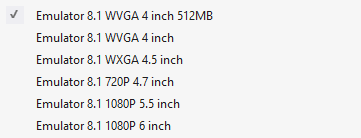
\includegraphics[resolution=120]{emulatory.png}
		\caption{Zestaw konfiguracji emulatorów dostępny w Windows Phone 8.1 SDK}
		\label{fig:emulatory}
\end{figure}

Aplikację przetestowałem na każdym z wyżej wymienionych urządzeń wirtualnych, a także na fizycznych urządzeniach: Nokia Lumia~925, Microsoft Lumia~530, Nokia Lumia~625.

Kopra została również uruchomiona w emulatorze systemu Windows 10 Mobile i działa poprawnie w konfiguracjach zaprezentowanych poniżej (rysunek \ref{fig:emulatoryWin10}). Nie została przetestowana dokładnie na nich. Podobnie nie miałem dostępu do urządzeń fizycznych z systemem Windows 10 Mobile, stąd użytkownik powinien używać oprogramowania na tym systemie na własną odpowiedzialność.

\begin{figure}[htp]
	\centering
			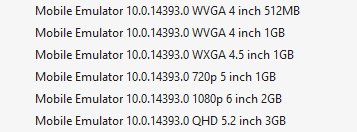
\includegraphics[resolution=120]{emulatoryWin10.png}
		\caption{Zestaw konfiguracji emulatorów dostępny w Windows 10 Mobile SDK}
		\label{fig:emulatoryWin10}
\end{figure}



\section{Newtonsoft.Json}

Newtonsoft.Json stanowi najpopularniejsze narzędzie do pracy z danymi w formacie JSON. Oprogramowanie działa na jednej z najbardziej liberalnych licencji, MIT.\cite{mitLicence} Wśród bibliotek dostępnych w menadżerze pakietów NuGet, zajmuje pierwsze miejsce mając ponad 15 milionów pobrań.[15] 

Json.NET znacznie uprościł proces przetwarzania danych otrzymanych z serwisu. Zgodnie z opisem zamieszczonym na stronie projektu, biblioteka jest bardzo łatwa w użyciu, nawet w przypadku złożonych typach danych. Znalazłem się jednak kilkukrotnie w sytuacji, gdy musiałem rozbudować mechanizm serializujący o dodatkowe warunki. Działo się tak kiedy serwis zwracał mi różne rodzaje danych dla jednego zapytania. 

Do pobierania elementów ze struktury HTML, których nie można pobrać przez API serwisu, istnieje mechanizm wspierający XPath. JSONPath \cite{jsonPath} jest wbudowany w bibliotekę i świetnie wspiera pobieranie elementów wg ścieżki oraz natychmiastowe serializowanie ich do formatu JSON.


\section{Git i GitHub}
W utrzymaniu ładu podczas pracy z kolejnymi wersjami aplikacji pomógł mi Git. Jest to rozproszony system kontroli wersji, stworzony przez Linusa Torvaldsa jako narzędzie do zarządzania kodem źródłowym Linuxa. Motywacją autora do napisania własnego systemu kontroli wersji było pogorszenie relacji z firmą BitMover, gdyż w efekcie projekt Linux stracił możliwość darmowgo korzystania z BitKeeper'a. 

Git został zaprojektowany w oparciu o 5~cech, które do dziś stanowią jego podstawę: szybkość, prosta konstrukcja, wsparcie dla równoległego rozwoju wielu wersji jednocześnie, w pełni rozproszony, z możliwością zarządzania wielkimi projektami.\cite{git}

Przekonującym argumentem do użycia właśnie tego systemu kontroli wersji jest dostęp do serwisów zintegrowanych z oprogramowaniem. Zmiany przechowywane są lokalnie w formie lokalnej bazy. Większość akcji wykonywanych na repozytorium Git to dodawanie danych do bazy. Sprawia to, że zniszczenie czegoś bez możliwości przywrócenia stanu jest prawie niemożliwe. Dzięki temu można śmiało dokonywać zmian w projekcie bez obaw o utratę danych. 

Tworząc większe funkcjonalności w projekcie korzystałem z możliwości tworzenia własnych gałęzi \textit{(branch)}, a następnie po zaimplementowaniu łączyłem je do głównej linii produkcyjnej \textit{(master)}.

Zamiast korzystać z własnego serwera systemu kontroli wersji, użyłem darmowego i najbardziej popularnego serwisu oferującego usługi przechowania repozytorium Git -- GitHub.com. Na chwilę obecną jest on największą platformą hostującą projekty open-source. Ponad 18~milionów użytkowników i 48~milionów założonych projektów pozwala twierdzić, że w trakcie tworzenia projektu serwis nie zostanie nagle wyłączony z użycia. Usługa oferuje możliwość przechowania kodu widocznego dla wszystkich \textit{(Public)} oraz tylko dla wybranych użytkowników \textit{(Private)}. GitHub jest darmowy dla pierwszego typu hostingu.\cite{gutHubCennik} 

Również kod źródłowy Kopry jest widoczny dla każdego -- jeśli ktoś zechce wykonać własną gałąź aplikacji i w jakikolwiek sposób ją poprawić, będzie to dla mnie miłym zaskoczeniem.


\section{LinqPad}
Narzędzie LinqPad wykorzystałem w celu szybkiego modelowania kodu metod. Jest to produkt powszechnie używany do modelowania fragmentów kodów w środowisku .NET. 

Zaletę programu stanowi możliwość pisania interaktywnych zapytań SQL z wykorzystaniem LINQ oraz pisania kodu C\# bez konieczności uruchamiania Visual Studio.\cite{linqPad} 

Produkt jest tworzony na modelu Freemium, co oznacza, że program jest darmowy z wyłączeniem pewnych funkcjonalności, za które należy zapłacić.\cite{linqPadWiki}



\section{ILSpy}
ILSpy to przeglądarka plików assembly i dekompilator kodu .NET, oparty o licencję MIT. Projekt hostowany jest na GitHub, gdzie można pobrać jego źródła.\cite{ilSpyRepo} 

Początkowo używałem tego narzędzia do dekompilacji biblioteki \textit{HtmlAgilityPack}, która przez wzgląd na zbyt wiele błędów zmusiła mnie do przeglądania jej wewnętrznych metod. Na późniejszym etapie ILSpy pomógł mi dokładniej zrozumieć część biblioteki .NET zawartej w przestrzeni nazw \texttt{System.Net.Http}. 

ILSpy stał się szczególnie popularny, kiedy narzędzie Microsoftu o nazwie IL DASM przestało stanowić część pakietu Visual Studio. Przed wersją Visual Studio 2012, IL~DASM był dostępny z poziomu folderu \textit{Microsoft SDK Tools} jako narzędzie udostępnione w zestawie razem z IL ASM. Ten zaś służy jako narzędzie do generowania kodu wykonywalnego z kodu pośredniego. Obecnie te narzędzia dostępne są w formie konsolowych programów. 

ILSpy jest w pełni graficznym narzędziem. Uważam, że stanowi najlepsze darmowe rozwiązanie dla przeglądania plików assembly.

 

\chapter{Budowa projektu}
Projekt został zbudowany w oparciu o bibliotekę Windows Phone SDK z wykorzystaniem wzorca architektonicznego MVVM. Z narzędzi zewnętrznych, zapewniłem integrację z Web API serwisu Kokos.

\section{Wzorzec MVVM}
W tym rozdziale przedstawię wzorzec architektoniczny MVVM, jego zalety i wady oraz sposób w jaki zaimplementowałem go w projekcie.

\subsection{Opis wzorca Model View ViewModel}

Wprowadzony przez Microsoft w 2005 roku, wzorzec architektoniczny, opiera się na tych samych założeniach co zaprezentowany lata wcześniej model prezentacji (Presetation Model). PM dziedziczy po Model Widok Prezenter MVP - \textit{(ang.Model View Presenter)}, wzorzec architektoniczny z początku lat 90 ubiegłego wieku. Z tym, że wzorzec PM jest szczególnie przydatny w programowaniu złożonych interfejsów użytkownika. Na systemie Windows, Presentation Model bardzo dobrze współpracuje z interfejsem użytkownika zbudowanym z biblioteką Windows Presentation Foundation (WPF) oraz biblioteką Silverlight. Właśnie dlatego Microsoft zbudował wersję wzorca PM specjalnie pod WPF i nazwał go Model-View-ViewModel (MVVM). \cite{aspNet} MVVM używa wielu specyficznych możliwości i narzędzi znanych z platformy Silverlight takich jak wiązanie danych. Wprowadzenie wzorca MVVM w aplikacjach opierających się na technologiach WPF, Silverlight jest zalecanym podejściem, ponieważ są to bardzo ułatwiają jego implementację.

Do zalet Model View ViewModel względem tradycyjnego podejścia (przeciągania kotrolek z Toolboxa i pisanie dalej w formie Code-behind) są:

\begin{itemize}

	\item Umożliwia oddzielenie logiki od sposobu wyświetlania. W dłuższej perspektywie ułatwia to rozwój, testowanie i utrzymanie kodu.
	\item Jest wspierany przez platformy XAML.
	\item Kod interfejsu jest niezależny od platformy kodu wykonywalnego.
	\item Umożliwia rozdział między projektanta interfejsu i programistę, tzn. każdy z nich może pracować oddzielnie nad swoją odpowiedzialnością.
\end{itemize}

Wzorzec podzielony jest na trzy części, które wspierają testowanie aplikacji przez rozdzielenie elementów interfejsu użytkownika od logiki aplikacji. Taki rozdział pozwala na wymianę komponentów aplikacji, wewnętrzną zmianę implementację, wyizolowane testy jednostkowe. Komponenty na najwyższym poziomie abstrakcji nie wiedzą o sobie zbyt wiele. Widok (V) wie o istnieniu \textbf{widok-modelu} \textit{(ang. ViewModel)} (VM), widok-model (VM) wie o istnieniu modelu, jednak model nie wie o widok-modelu (VM) i widok-model (VM) nie wie nic o Widoku (V).

\begin{description}

	\item[Widok \textit{(View)}] odpowiada za strukturę, rozkład i wygląd tego co użytkownik otrzymuje na ekranie. W większości przypadków aplikacji Windows Phone, widok zdefiniowany jest jako Strona zaimplementowana przy użyciu XAML’a. Widok ma kilka możliwości na wykonanie kodu dla użytkownika, najczęściej rekomendowanym sposobem jest użycie właściwości \textit{Command}.
	
	\item[Model \textit{(Model)}] jest odpowiedzialny za przechowywanie danych w obrębie swojej domeny oraz logiki biznesowej.
	
	\item[Widok-model \textit{(ViewModel)}] rozdziela logikę biznesową od widoku. Zadaniem tego komponentu jest pobranie danych z Modelu i przedstawienie go w formie łatwo przyswajalnej dla widoku. Widok-model również może odpowiadać za stany widoku, jak na przykład przekazanie widokowi stanu ładowania.

\end{description}


\subsection{MVVM vs MVC}

Praca nie byłaby kompletna, gdybym nie wspomniał nic o wzorcu, który wpłynął w znaczący sposób na rozwój MVVM. Wzorzec bardzo podobny, który powstał jednak dużo wcześniej to Model-View-Controller (MVC). Jest to wzorzec architektoniczny, używany do implementacji interfejsu użytkownika. Polega na podziale oprogramowania na trzy niezależne od siebie części. Wzorzec został zaprezentowany po raz pierwszy przez Trygve Reenskaug jeszcze w latach 70tych. \cite{mvcXerox} Wzorzec dzieli modelowanie domeny, prezentacji i akcji na trzy oddzielne klasy. Model zarządza zachowaniem i danymi w domenie aplikacji, odpowiada na żądania informacji o swoim stanie oraz odpowiada na żądania zmiany stanu, które otrzyma od kontrolera. View stanowi o graficznej części aplikacji, otrzymuje od kontrolera informacje w jaki sposób interpretować dane wejściowe otrzymane od użytkownika. Controller służy do przetwarzania informacji otrzymywanych od użytkownika np. z urządzeń wejściowych. MVC stał się bardzo popularnym wzorcem przy projektowaniu aplikacji typu desktop, a później także Web. 


\subsection{Implementacja MVVM w aplikacji}
Aplikacje korzystające z wzorca MVVM mają z góry ustalony szkielet folderów.

\begin{figure}[h]
	\centering
			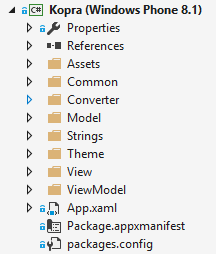
\includegraphics[resolution=120]{strukturaFolderow.png}
		\caption{Struktura folderów w projekcie aplikacji Kopra}
\end{figure}

Mój projekt ściśle trzyma się tej struktury wraz z dodatkowymi elementami. Przyjąłem następującą konwencje nazewniczą, dla każdego widoku dołączyłem sufiks ,,Page'', natomiast każdy widok-model w nazwie ma dołączony sufiks ,,ViewModel''. Każdy widok ma odpowiadający mu jeden widok-model. 


\begin{figure}[h]
	\centering
	\begin{minipage}[h]{0.3\textwidth}
		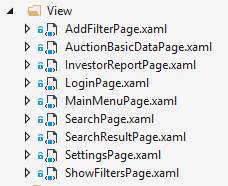
\includegraphics[width=\textwidth]{listawidokow.png}
		\caption{Lista plików widoków w projekcie}
	\end{minipage}
\hspace*{60px}
	\begin{minipage}[h]{0.3\textwidth}
		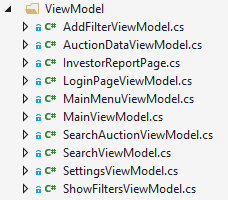
\includegraphics[width=\textwidth]{listaviewmodeli.png}
		\caption{Lista plików widok-modeli w projekcie}
	\end{minipage}
	\hfill
\end{figure}


%Podpięcie widok-modelu do Widoku w pliku XAML: 
\noindent
\begin{minipage}{\linewidth}
\begin{lstlisting}[caption=Podpięcie widok-modelu do Widoku w pliku XAML, label=lst:test, language=xml]
<Page.DataContext>
	<viewModel:NameViewModel></viewModel:NameViewModel>
</Page.DataContext>
\end{lstlisting}
\end{minipage}

%Podpięcie widok-modelu w pliku Code-Behind:

\noindent
\begin{minipage}{\linewidth}
\begin{lstlisting}[caption=Podpięcie widok-modelu w pliku Code-Behind, label=lst:test]
private AddFilterViewModel _viewModel;

public AddFilterPage() 
{
	_viewModel = DataContext as AddFilterViewModel;
}
\end{lstlisting}
\end{minipage}


\noindent
\begin{minipage}{\linewidth}

Do wiązania danych zaimplementowałem interfejs INotifyPropertyChanged. 

\begin{lstlisting}[caption=Implementacja interfejsu INotifyPropertyChanged w jednej z klas, label=lst:test]
public class MainViewModel : INotifyPropertyChanged
{
	public event PropertyChangedEventHandler PropertyChanged;
	
	public void NotifyPropertyChanged(string propertyName)
	{
		PropertyChanged?.Invoke(this,
			new PropertyChangedEventArgs(propertyName));
	}
}
\end{lstlisting}
\end{minipage}

Mając tak zaimplementowaną klasę, pozostałe widok-modele dziedziczą po MainViewModel używając wywołania metody \textit{NotifyPropertyChanged()} do powiadomienia o zmianie wartości właściwości.

\noindent
\begin{lstlisting}[caption=Przykładowa właściwość wykorzystująca mechanizm NotifyPropertyChanged, label=lst:test]
public string ApiKeyValue
{
	get { return _apiKeyValue; }
	set
	{
		_apiKeyValue = value;
		NotifyPropertyChanged(nameof(ApiKeyValue));
	}
}
\end{lstlisting}

\section{Kokos WebAPI}

Rozdział przeznaczony na prezentację interfejsu programistycznego udostępnionego przez zespół BlueMedia. Przedstawiam również niedogodności związane z jego wykorzystaniem, metodę konsumpcji przez Koprę i sposoby poprawienia komfortu użytkowania. Przez rozpoczęciem pracy jedynym wymogiem (oprócz aktywnego konta) jest wygenerowanie klucza, który służy pozwala odróżnić kto wykonuje zapytanie.

\subsection{Opis interfejsu webowego}

Zapytania do serwisu wykonuje się przez złożenie zapytania RESTowego. Czyli 

\begin{center}
\texttt{https://kokos.pl/webapi/\textit{FUNKCJA}?key=\textit{KLUCZ}\&type=\textit{FORMAT\_DANYCH}\&\textit{PARAMETR}=\textit{WARTOŚĆ}}
\end{center}

Aby uniknąć nadmiernego obciążenia i wykorzystania klucza przez więcej niż jednego użytkownika liczba zapytań jest ograniczona do jednego na sekundę. Przy próbie przekroczenia, zostanie zwrócony w odpowiedzi kod 503. Lista dostępnych funkcji:

\begin{description}[style=nextline]

	\item[get-auction-data] Pobranie szczegółowych danych jednej wybranej aukcji.
	\item[get-auctions-by-status] Pobranie listy pożyczek według statusu.
	\item[search] Wyszukiwanie aukcji według podanych parametrów.
	\item[get-most-popular-auctions] Pobranie najbardziej popularnych aukcji.
	\item[get-recent-auctions] Pobranie ostatnio założonych aukcji.
	\item[get-recent-payments] Pobranie ostatnich wpłat za raty.
	\item[get-recent-investments] Pobranie najnowszych inwestycji.
	\item[get-ended-auctions-amount] Pobranie sumy wartości aukcji zakończonych sukcesem.
	\item[get-service-stats] Pobranie statystyk serwisu.
	\item[get-user-id-by-nick] Pobranie ID użytkownika na podstawie jego nick-u.
	\item[get-payment-stats] Pobranie statystyk spłacalności dla całego serwisu.
	\item[get-vindication-stats] Pobranie statystyk spłacalności.

\end{description}

Każda z funkcji ma określony spory zakres parametrów oraz tabelę ze zwracanymi wartościami. 


\subsection{Implementacja API w aplikacji}

W celu uniknięcia powielania kodu podczas zapytań, napisałem klasę, która generuje zapytania do serwisu. Wykorzystuje mniej niż 50\% funkcji, dlatego nie widziałem powodu by tworzyć osobny projekt na komunikację z serwisem. Elementy stałe, przechowuję w formie prywatnych elementów klasy.

\noindent
\begin{lstlisting}[caption=Składowe budujące zapytanie do serwisu, label=lst:test]
private const string BaseAddress = "https://kokos.pl/webapi/";
private const string DataType = "&type=json";
private const string Search = "search?";
private const string RecentAuctions = "get-recent-auctions?";
private const string AuctionData = "get-auction-data?";
private const string Comments = "comments=1";
private const string Records = "records=";
private const string Key = "key=";
private const string Id = "id=";
private const string Type = "type=";
\end{lstlisting}


Tworzenie parametrów zapytań API schowane jest w klasie RequestGenerator. Przechowuje tam zbiór funkcji do tworzenia całościowych obiektów Uri, gotowych do przekazania użycia przez serwis.

\noindent
\begin{lstlisting}[caption=Nagłówki metod pozwalających składać zapytania do serwisu., label=lst:test]
public Uri FilteredAuction(string filter)
public Uri ComposeSearchAuctionQuery(Dictionary<string, string> search)
public Uri MostRecentAuctions()
public Uri GetAuctionData(GetAuctionDataParameters parameters)
\end{lstlisting}

Komunikacja z serwisem odbywa się przy pomocy klasy KokosConnectionManager. Do komunikacji internetowej, wykorzystana jest klasa HttpClient.


\section{Notyfikacje przez BackgroundTask}


\subsection{Opis}

Windows Phone 8.1 pozwala wykonywać aplikacji zadania bez konieczności trzymania jej na pierwszym tle. Funkcjonalność ta nazywa się \textit{Background Task} i użyłem jej do powiadamiania użytkownika o nowych aukcjach w serwisie.

\subsection{Implementacja NewAuctionNotifier}

{\color{red}\textit{Lorem ipsum dolor sit amet, consectetur adipiscing elit. Curabitur non lectus pulvinar, bibendum est eu, venenatis odio. In faucibus orci vel tortor pellentesque molestie. Nullam vel risus mattis, volutpat arcu non, cursus est. Phasellus facilisis risus id justo consectetur porta. Integer neque lorem, tincidunt in mi id, eleifend consequat quam. Sed lacinia feugiat neque. Sed id eleifend lectus, et vulputate enim. Aenean viverra, diam vitae sodales auctor, risus risus varius metus, vitae bibendum metus nibh et ipsum. Aenean id placerat neque. }}





\chapter{Prezentacja interfejsu aplikacji}

\section{Etymologia nazwy}

Nazwa aplikacji powstała już w trakcie tworzenia, kiedy wiedziałem już z którym serwisem aplikacja będzie współpracować. Szukałem czegoś co jednym słowem opisze sposób myślenia inwestora. \textit{,,Jak wyciągnąć największe zyski z inwestycji?''}. W połączeniu z nazwą serwisu, który obsługuje, nie mogło być lepszej nazwy jak Kopra. Co miało podkreślić, wyciągnięcie esencji z Kokosa.

\section{Korzyści względem wersji przeglądarkowej}

Ze względu na brak dobrej przeglądarki internetowej w urządzeniach Windows Phone, stronę trudno jest obsługiwać z poziomu telefonu. Sam serwis nie jest dostosowany do małych ekranów urządzeń mobilnych (brak poprawnie zaimplementowanej responsywności). Kopra została zaprojektowana wyłącznie na takie urządzenia i jest to największa jej zaleta w stosunku do strony internetowej. 


\section{Koszt użytkowania aplikacji}

Aplikacja jest darmowa, również wersja, która zostanie wystawiona do sklepu będzie udostępniona bezpłatnie, bez reklam. To jest największa różnica względem konkurencyjnego oprogramowania Kokoid, które na każdym ekranie wyświetla użytkownikowi baner reklamowy. Kod źródłowy aplikacji jest dostępny w oparciu o liberalną licencję MIT.

\section{Bezpieczeństwo danych przechowywanych w aplikacji}

Aplikacja ma po zalogowaniu ma dostęp do wszystkich danych osobowych umieszczonych w serwisie. Do tych danych należą między innymi: numer i seria dowodu osobistego, adres użytkownika, adresy IP z datą logowania do serwisu, historia kredytowa, aktualne inwestycje, saldo użytkownika, hasło oraz email. Z całego ogromu informacji, w aplikacji trzymane są tylko dane logowania i klucz dostępu do WebAPI użytkownika. Aby poprawić bezpieczeństwo, cały ruch między aplikacją a serwisem Kokos jest przesyłany protokołem SSL. Również aby zapobiec ewentualnym wyciekom danych, aplikacja nie wysyła danych logowania na serwery zewnętrzne.

\section{Jak wygląda Kopra?}

\subsection{Logo}

Logo aplikacji jest rysunkiem połowy owocu kokosowego z liśćmi drzewa kokosowego. Jak wspomniałem w pierwszych rozdziałach pracy, jest to nawiązanie nazwy do wykorzystywanego serwisu. Logo zostało wykonane w bieli, bez tła, dlatego jest przystosowane do każdego motywu kolorystycznego z nasyconymi barwami (różnymi od bieli).

\begin{figure}[h]
	\centering
	\begin{minipage}[b]{0.3\textwidth}
		
\includegraphics[width=\textwidth]{kafelekSzeroki.png}
		\caption{Logo na szerokim kafelku}
	\end{minipage}
\hspace*{60px}
	\begin{minipage}[b]{0.3\textwidth}
		
\includegraphics[width=\textwidth]{kafelekKwadratowy.png}
		\caption{Logo na kwadratowym kafelku}
	\end{minipage}
	\hfill
\end{figure}


\subsection{Splash screen}


W trakcie uruchamiania aplikacji, użytkownik może zobaczyć duże logo aplikacji wraz z jej nazwą na niebieskim tle. 
\begin{figure}[h]
	\begin{minipage}[h]{\textwidth}
		\centering
		
\includegraphics[width=0.3\textwidth]{splashScreen.png}
		\caption{Splash screen}
	\end{minipage}
	\hfill
\end{figure}


\subsection{Strona logowania}
Pierwszy ekran jaki widzi użytkownik, jest on wykonany w motywie pośrednim. Pozwala na łagodne przejście między domyślnym ciemnym motywem Windows Phone na motyw jasny, który będzie widoczny po zalogowaniu się do serwisu. Na tym ekranie użytkownik jest zmuszony do przekazania loginu (adresu email) oraz hasła bezpośrednio do strony Kokos.pl. Po wybraniu przycisku zaloguj, jest on zastąpiony przez napis ,,Logowanie...'' oraz animację paska postępu. Dodatkowym elementem są komunikaty informujące użytkownika np. o braku połączenia z Internetem.
\begin{figure}[h]
	\begin{minipage}[h]{\textwidth}
		\centering
		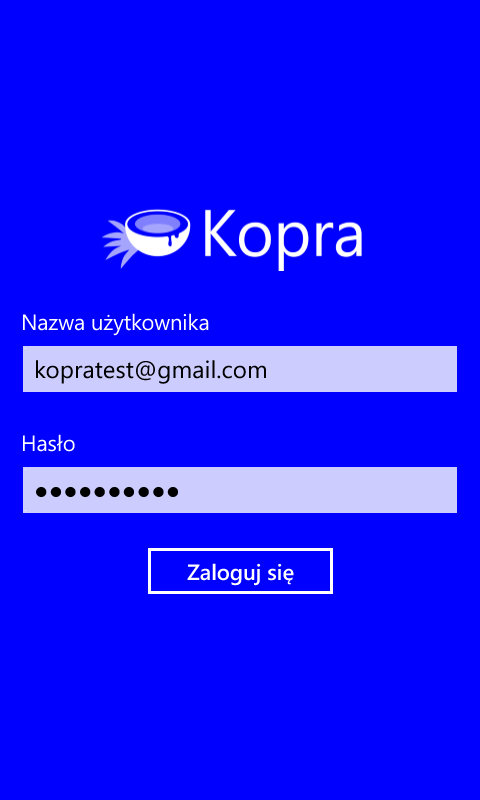
\includegraphics[width=0.3\textwidth]{logowanie.png}
		\caption{Ekran logowania}
	\end{minipage}
	\hfill
\end{figure}


\subsection{Strona główna}
Ekran dostępny po zalogowaniu składa się z trzech części. Na górze ekranu po lewej stronie widnieje mała wersja logo oraz nazwy aplikacji. Po prawej stronie, znajduje się nazwa zalogowanego użytkownika. Drugą część stanowią przyciski, symulujące wyglądem kafelki znane w ekosystemie Windows Phone 8. Jest to miejsce agregujące najważniejsze funkcje dostępne dla użytkownika. 
\begin{figure}[h]
	\begin{minipage}[h]{\textwidth}
		\centering
		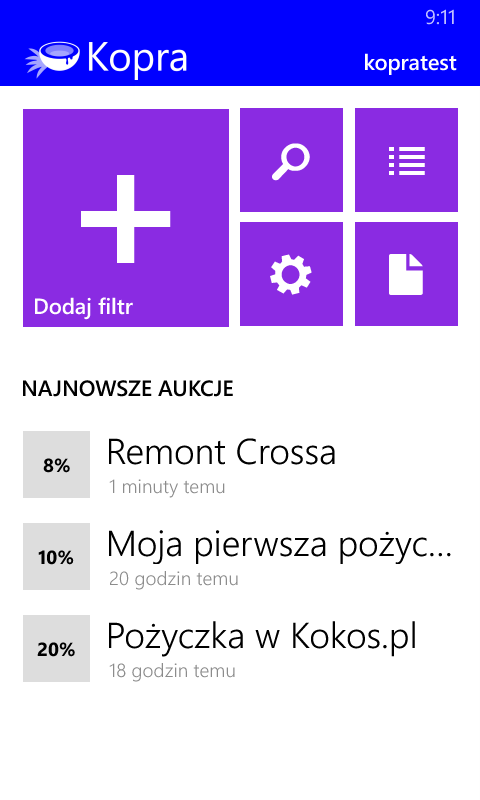
\includegraphics[width=0.3\textwidth]{mainScreen.png}
		\caption{Strona główna aplikacji}
	\end{minipage}
	\hfill
\end{figure}

\subsection{Dodaj filtr}
Ekran znajduje się pod przyciskiem \textit{Dodaj filtr} z ikoną znaku plus na stronie głównej aplikacji. Jest on przeznaczony do dodawania kryteriów wyszukiwania w postaci plików w pamięci telefonu.

\section{Instrukcja obsługi do aplikacji}

Aby korzystać z aplikacji, należy mieć aktywne konto w serwisie kokos.pl oraz aktywować klucz API pierwszy raz przez przeglądarkę. Po uruchomieniu Kopry, należy podać adres email oraz hasło logowania do serwisu. Po poprawnej weryfikacji, użytkownik zostanie przeniesiony do ekranu głównego, skąd może się dostać do wszystkich najważniejszych funkcjonalności aplikacji. Użytkownik może przeskoczyć bezpośrednio do jednej z trzech najnowszych aukcji wyświetlanych na dole ekranu.

Aby uruchomić zadania w tle, należy mieć dodany przynajmniej jeden filtr w aplikacji, a następnie z ekranu ustawień wybrać z listy, jakie aukcje mają być wyszukiwane w tle. Maksymalnie co 30 minut można otrzymać powiadomienie, z nową aukcją.

 
\chapter{Podsumowanie}
Aplikacja ma w założeniu rozwiązać problem, jakim jest szybki dostęp do oferty pożyczkowej na urządzeniach mobilnych. Skupia się na obsłudze najpopularniejszego serwisu, oferującego usługi ,,p2p lending''. Kopra ma wyciągnąć najważniejsze informacje, potrzebne do dalszego procesu myślowego czy warto zainteresować się ofertą. 

Wymuszenie jasnego motywu, miało pomóc w zdobyciu zaufania użytkownika oraz nadać czystą strukturę interfejsowi. Aby lepiej poznać nawyki użytkowników systemu Windows Phone, zdecydowałem się na użytkowanie systemu przez rok, równolegle z procesem pisania pracy. Jest to główny powód zmiany interfejsu po pierwszej iteracji, gdzie ekrany przypominały zmniejszoną wersję przeglądarkową serwisu. Ze względu na ogrom danych dostępnych użytkownikowi w serwisie, zdecydowałem się na zaprezentowanie szczegółów aukcji na ekranie typu pivot, który pozwala na łatwe grupowanie informacji powiązanych ze sobą tematycznie. 
Oprogramowanie stworzyłem z myślą o telefonach Windows Phone 8.1 wraz z kolejnymi wersjami, ponieważ jest to system stworzony z myślą o produktywności, szczególnie pod kątem ludzi biznesu. 

Na chwilę obecną aplikacja ma możliwość sprawdzania w tle jednego filtru użytkownika. Funkcjonalność można rozszerzyć o wybór ilości powiadomień na godzinę, które użytkownik jest w stanie zaakceptować, dodać listę filtrów które miałyby być sprawdzane i ustawić dla nich priorytety. Również widzę w kolejnych wersjach możliwość tworzenia kopii zapasowej filtrów na dysku OneDrive oraz dzielenie się nimi z innymi inwestorami. Kolejnym kamieniem milowym w rozwoju aplikacji może być automat inwestycyjny, który korzystając z funkcjonalności wyszukiwania aukcji w tle, inwestowałby automatycznie określoną kwotą w znalezione oferty inwestycyjne.

Stworzona przeze mnie aplikacja jest pierwsza w swojej kategorii. Liczę na odzew programistów po publikacji Kopry w Sklepie Microsoft. Zależy mi by inwestowanie przez Koprę było łatwą formą pomnażania oszczędności, bez płacenia wysokich prowizji pośrednikom, co pomoże poprawić domowy budżet wielu osób.
 
 
 
 
\addcontentsline{toc}{chapter}{Spis rysunków}
\listoffigures


\addcontentsline{toc}{chapter}{Bibliografia}
\begin{thebibliography}{99}

\bibitem{git} \textsc{Chacon S., Straub B.:}
\textit{Pro Git}, Apress, 2014, Wydanie II, ISBN 978-14-842-0077-3.

\bibitem{aspNet} \textsc{Dino E.:}
\textit{Programming Microsoft ASP.NET 4}, Microsoft Press, 2011, \\ISBN~978-0-7356-4338-3.

\bibitem{inwestycje} \textsc{Jajuga K., Jajuga T.:}
\textit{Inwestycje. Instrumenty finansowe, ryzyko finansowe, inżynieria finansowa}, Warszawa, Wydawnictwo Naukowe PWN SA, 2015, Wydanie III zm., \\ISBN 978-83-01-14957-4.

\bibitem{slownikPwn} \textsc{Drabik L., Sobol	E.:}
\textit{Słownik języka polskiego PWN}, Wydawnictwo Naukowe PWN, 2007, ISBN 978-8-3011-7377-7.

\bibitem{slownikNBP} \textit{Słownik serwisu NBP - Portal Edukacji Ekonomicznej}, \\
\texttt{https://www.nbportal.pl/slownik/pozycje-slownika/toksyczne-aktywa}, \\dostęp: 05.01.2017.

\bibitem{soros} \textit{Billionaire who broke the Bank of England}, 
\texttt{http://www.telegraph.co.uk/finance/2773265/\\Billionaire-who-broke-the-Bank-of-England.html}, dostęp: 27.12.2016.

\bibitem{wpDesign} \textit{Design Universal Windows Platform (UWP) app}, 
\texttt{https://dev.windows.com/en-us/design}, dostęp: 27.12.2016.

\bibitem{doMore} \textit{DoMore Archives}, 
\texttt{http://blogs.microsoft.com/firehose/tag/DoMore/}, \\dostęp: 27.12.2016.

\bibitem{financingCivilization} \textit{Financing Civilization}, 
\texttt{http://viking.som.yale.edu/will/finciv/chapter1.htm}, \\dostęp: 27.12.2016.

\bibitem{fractionalReserveBanking} \textit{Fractional Reserve Banking -- An Economist's Perspective (Transcript)}, \\
\texttt{https://www.frbatlanta.org/education/classroom-economist/\\fractional-reserve-banking/economists-perspective-transcript}, dostęp: 27.12.2016.

\bibitem{P2P} \textit{Taking a Peek at Peer-to-Peer Lending}, 
\texttt{http://business.time.com/2012/11/15/\\taking-a-peek-at-peer-to-peer-lending/}, dostęp: 27.12.2016.

\bibitem{antybelkowe} \textit{Koniec lokat antybelkowych. Co w zamian}, 
\texttt{http://www.money.pl/pieniadze/\\wiadomosci/artykul/koniec;lokat;antybelkowych;co;w;zamian,82,0,1057874.html}, dostęp: 27.12.2016.

\bibitem{nsaZnamiona} \textit{Wyrok NSA, sygn. II FSK 1472/10}, \texttt{http://orzeczenia.nsa.gov.pl/doc/1F82F6552C}, \\dostęp: 27.12.2016.

\bibitem{nsaWyrokOdwrotny} \textit{Wyrok NSA, sygn. II FSK 142/10}, 
\texttt{http://orzeczenia.nsa.gov.pl/doc/862AF4722F}, \\dostęp: 27.12.2016.

\bibitem{oswiadczenieKokos} \textit{Oświadczenie Zespołu Kokos.pl w sprawie wyroku NSA o sygn. II FSK 1472/10}, \\
\texttt{https://kokos.pl/aktualnosci/czytaj?id=2012\_03\_06}, dostęp: 27.12.2016.

\bibitem{zostanInwestorem} \textit{Zostań Inwestorem -- Kokos.pl}, 
\texttt{https://kokos.pl/info/chce-inwestowac}, \\dostęp: 28.10.2016.

\bibitem{stopy} \textit{Podstawowe stopy procentowe NBP}, 
\texttt{http://www.nbp.pl/home.aspx?f=/dzienne/stopy.htm}, \\dostęp: 27.12.2016.

\bibitem{finansowoPl} \textit{Pożyczki społecznościowe finansowo.pl}, 
\texttt{https://www.finansowo.pl}, dostęp: 27.12.2016.

\bibitem{zakraPl} \textit{Pożyczki społecznościowe zakra.pl}, 
\texttt{https://zakra.pl}, dostęp: 27.12.2016.

\bibitem{kokosPl} \textit{Pożyczki społecznościowe kokos.pl}, 
\texttt{https://kokos.pl}, dostęp: 27.12.2016.

\bibitem{lendicoPl} \textit{Pożyczki społecznościowe lendico.pl}, 
\texttt{https://www.lendico.pl}, dostęp: 27.12.2016.

\bibitem{zakraminiPl} \textit{Pożyczki społecznościowe zakramini.pl}, 
\texttt{https://zakramini.pl}, dostęp: 27.12.2016.

\bibitem{applecreditPl} \textit{Pożyczki społecznościowe applecredit.pl}, 
\texttt{https://applecredit.pl}, dostęp: 27.12.2016.

\bibitem{capitalclubPl} \textit{Pożyczki społecznościowe capitalclub.pl}, 
\texttt{https://capitalclub.pl}, dostęp: 27.12.2016.

\bibitem{zakraPlApi} \textit{Funkcje webAPI serwisu Zakra.pl}, 
\texttt{https://zakra.pl/api}, dostęp: 27.12.2016.

\bibitem{kokosPlApi} \textit{Dokumentacja WebAPI serwisu Kokos.pl}, 
\texttt{https://kokos.pl/webapiinfo/dokumentacja}, dostęp: 08.11.2015.

\bibitem{vs} \textit{Microsoft Visual Studio Community 2015}, \\
\texttt{https://www.microsoft.com/en-us/download/details.aspx?id=48146}, \\dostęp: 27.12.2016.

\bibitem{csharp} \textit{Dokumentacja języka C\# dla Visual Studio 2015}, \\
\texttt{https://msdn.microsoft.com/en-us/library/kx37x362.aspx}, \\dostęp: 27.12.2016.

\bibitem{dotnetArtykul} \textit{Komponenty architektury zestawu narzędzi .NET}, \\
\texttt{https://docs.microsoft.com/en-us/dotnet/articles/standard/components},\\ dostęp: 27.12.2016.

\bibitem{tajneArchiwaMicrosoftu} \textit{Archiwum Windows SDK oraz emulatorów}, \\
\texttt{https://developer.microsoft.com/en-us/windows/downloads/sdk-archive}, \\dostęp: 27.12.2016.

\bibitem{mitLicence} \textit{Treść licencji MIT wykorzystywanej przez Newtonsoft.Json}, \\
\texttt{https://github.com/JamesNK/Newtonsoft.Json/blob/master/LICENSE.md}, \\dostęp: 27.12.2016.

\bibitem{jsonPath} \textit{Strona domowa projektu JsonPath}, 
\texttt{http://goessner.net/articles/JsonPath/}, \\dostęp: 27.12.2016.

\bibitem{gutHubCennik} \textit{Plany abonamentowe serwisu GitHub.com}, 
\texttt{https://github.com/pricing}, \\dostęp: 27.12.2016.

\bibitem{linqPad} \textit{LINQPad as a Code Scratchpad}, 
\texttt{http://www.linqpad.net/CodeSnippetIDE.aspx}, \\dostęp: 27.12.2016.

\bibitem{linqPadWiki} \textit{Opis LINQPad na Wikipedii}, 
\texttt{https://en.wikipedia.org/wiki/LINQPad}, \\dostęp: 27.12.2016.

\bibitem{ilSpyRepo} \textit{Repozytorium projektu ILSpy}, 
\texttt{https://github.com/icsharpcode/ILSpy}, \\dostęp: 27.12.2016.

\bibitem{mvcXerox} \textit{Oryginalna notka techniczna nt. wzorca MVC stworzona dla XEROX PARC w latach 1978-79}, \\
\texttt{http://heim.ifi.uio.no/~trygver/themes/mvc/mvc-index.html}, \\dostęp: 27.12.2016.



\end{thebibliography}




\end{document}
